% !TEX program = pdflatex
% !TEX options = -synctex=1 -interaction=nonstopmode -file-line-error "%DOC%"
% 作业模板
\documentclass[UTF8,10pt,a4paper]{article}
\usepackage{ctex}
\newfontfamily\menlo{MONACO.TTF}
\usepackage{amsmath}
\usepackage{diagbox}
\usepackage{float}
\usepackage{listings}
\usepackage{multirow}
\usepackage{tabularx}

\usepackage{url}
\usepackage{xcolor}
\newcommand{\tabincell}[2]{\begin{tabular}{@{}#1@{}}#2\end{tabular}}

\lstset{
    breaklines,                                 % 自动将长的代码行换行排版
    extendedchars=false,                        % 解决代码跨页时,章节标题,页眉等汉字不显示的问题
    backgroundcolor=\color[rgb]{0.96,0.96,0.96},% 背景颜色
    keywordstyle=\color{blue}\bfseries,         % 关键字颜色
    identifierstyle=\color{black},              % 普通标识符颜色
    commentstyle=\color[rgb]{0,0.6,0},          % 注释颜色
    stringstyle=\color[rgb]{0.58,0,0.82},       % 字符串颜色
    showstringspaces=false,                     % 不显示字符串内的空格
    numbers=left,                               % 显示行号
    numberstyle=\tiny\menlo,                    % 设置数字字体
    basicstyle=\small\menlo,                    % 设置基本字体
    captionpos=t,                               % title在上方(在bottom即为b)
    frame=single,                               % 设置代码框形式
    rulecolor=\color[rgb]{0.8,0.8,0.8},         % 设置代码框颜色
}  

\usepackage{pythonhighlight}
\usepackage{listings}
\usepackage{xcolor}
\usepackage{graphicx}
\usepackage[a4paper,left=2cm,right=2cm,top=2cm,bottom=2cm]{geometry}
\usepackage{fancyhdr}
% \catcode`\。=\active
% \newcommand{。}{.}
\newcommand{\CourseName}{操作系统(Operating System)}
\newcommand{\CourseCode}{CS307 \& CS356}
\newcommand{\Semester}{2020-2021学年第二学期}
\newcommand{\ProjectName} {\Huge{Project 3}} 
\newcommand{\StudentName}{刘涵之}
\newcommand{\StudentID}{519021910102}
\usepackage[vmargin=1in,hmargin=.5in]{geometry}
\usepackage{fancyhdr}
\usepackage{lastpage}
\usepackage{calc}
\pagestyle{fancy}
\fancyhf{}
\fancyhead[L]{\CourseName}
\fancyhead[C]{\ProjectName}
\fancyhead[R]{\StudentName}
\fancyfoot[R]{\thepage\ / \pageref{LastPage}}
\setlength\headheight{12pt}
\fancypagestyle{FirstPageStyle}{
    \fancyhf{}
    \fancyhead[L]{\CourseName\\
        \CourseCode\\
        \Semester}
    \fancyhead[C]{\large\bfseries\ProjectName \\}
    \fancyhead[R]{Name: \makebox[\widthof{\StudentID}][s]{\StudentName}\\
        ID : \StudentID\\
        }
    \fancyfoot[R]{\thepage\ / \pageref{LastPage}}
    \setlength\headheight{36pt}
}
\usepackage{amsmath,amssymb,amsthm,bm}
\allowdisplaybreaks[4]
\newtheoremstyle{Problem}
{}
{}
{}
{}
{\bfseries}
{.}
{ }
{第\thmnumber{ #2}\thmname{ #1}\thmnote{ (#3)} 得分: \underline{\qquad\qquad}}
\theoremstyle{Problem}
\newtheorem{prob}{题}
\newtheoremstyle{Solution}
{}
{}
{}
{}
{\bfseries}
{:}
{ }
{\thmname{#1}}
\makeatletter
\def\@endtheorem{\qed\endtrivlist\@endpefalse}
\makeatother
\theoremstyle{Solution}
\newtheorem*{sol}{解}
\title{Project 3: Multithreaded Sorting Application and Fork-Join Sorting Application}
\date{}
% \usepackage{graphicx}
\begin{document}
\maketitle
\thispagestyle{FirstPageStyle}

\section{Multithreaded Sorting Application}
Write a multithreaded sorting program that works as follows: A list of integers is divided into two smaller lists of equal size. Two separate threads (which we will term \textbf{\textit{soring threads}}) sort each sublist using a sorting algorithm of your choice. The two sublists are merged by a third thread - a \textbf{\textit{merging thread}} - which merges the two sublists into a single sorted list.

Because global data are shared across all threads, perhaps the easiest way to set up the data is to create a global array. Each sorting thread will work on one half of this array. A second global array of the same size as the unsorted integer array will also be established. The merging thread will then merge the two sublists into this second array. Graphically, this program is structured as follows (Fig. \ref{fig1}).

This programming project will require passing parameters to each of the
sorting threads. In particular, it will be necessary to identify the starting index from which each thread is to begin sorting. The parent thread will output the sorted array once all sorting threads have exited.

\begin{figure}[H]
  \centering
  % Requires \usepackage{graphicx}
  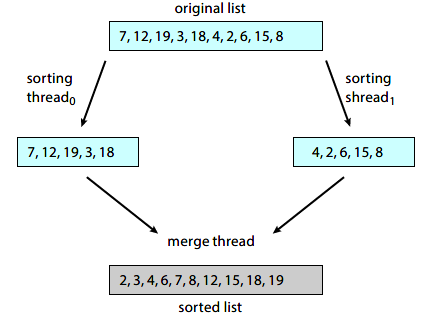
\includegraphics[width=4in]{fig1.png}\\
  \caption{Multithreaded sorting}\label{fig1}
\end{figure}

\textbf{Design}: My design for this task is shown as follows:
\begin{itemize}
    \item Global array \texttt{array} and \texttt{result} are shared between all thread.
    \item First, create two threads to sort \texttt{array}. Each thread sorts a subset of the whole \texttt{array}.
    \item Then, \textbf{sort\_thread()} function is designed to sort \texttt{array} from index \textbf{start} to index \textbf{end}. Index \textbf{start} to index \textbf{end} will be passed to it when the thread is created.
    \item After two sorting threads are finished (after we join them in the main()). \textbf{merge\_thread()} function is used to create a thread that merge the sorting result to \texttt{result}.
    \item The length of \texttt{array} is given by the user and the data is generated by \textbf{rand()} function.
\end{itemize}

The code for this task is shown as follows.
\begin{lstlisting}[language = c]
#include <pthread.h>
#include <stdlib.h>
#include <stdio.h>
#include <time.h>

int *array;
int *result;

struct function_args {
    int start, end, mid;
};

int cmp(const void *a, const void *b) {
	return *((int *)a) - *((int *)b);
}

void* sort_thread(void *arg) {
    struct function_args * args = (struct function_args *)arg;
    int start = args -> start;
    int end = args -> end;
    if (start > end) return NULL;
    
    qsort(array + start, end - start + 1, sizeof(int), cmp); // sort.

    return NULL;
}

void* merge_thread(void *arg) {
    struct function_args * args = (struct function_args *)arg;
    int start = args -> start;
    int mid = args -> mid;
    int end = args -> end;
    
    int loc1, loc2, i;
    loc1 = start;
    loc2 = mid + 1;
    i = 0;
    
    while (i <= end) {
        int flag = 1; // select which sub-array
        if (loc1 <= mid && (array[loc1] < array[loc2])) flag = 0;
        if (loc1 > mid) flag = 1;
        if (loc2 > end) flag = 0;
        if (flag == 0) {
            result[i++] = array[loc1++];
        } else {
            result[i++] = array[loc2++];
        }
    }
    return NULL;
}


int main() {
    int n;
    printf("Input the length of array:");
    scanf("%d", &n); // get the length of array.
    
    array = (int *) malloc (n * sizeof(int)); // allocate memory.
    result = (int *) malloc (n * sizeof(int));
    
    srand((unsigned int)time(0));
    printf("Array: [ "); // generate random array and print it.
    for(int i = 0; i < n; i++) {
        array[i] = rand() % 100;
        printf("%d ", array[i]);
    }
    printf("]\n");

    int start, mid, end; // divide array into two sub-array.
    start = 0;
    mid = n / 2;
    end = n - 1;

    struct function_args args[2]; // arguments for sort threads.
    args[0].start = start;
    args[0].end = mid;
    args[1].start = mid + 1;
    args[1].end = end;

    pthread_t sort_th[2]; // create 2 sort thread to sort sub-array.
    for (int i = 0; i < 2; i++) {
        if (pthread_create(&sort_th[i], NULL, sort_thread, &args[i])) {
            printf("Can't create thread.\n");
            return 1;
        }
    }

    for (int i = 0; i < 2; i++) { // join 2 sort thread.
        void *out;
        if (pthread_join(sort_th[i], &out)) {
            printf("Can't join thread.\n");
            return 1;
        }
    }
    
    args[0].start = start; // arguments for merge thread.
    args[0].mid = mid;
    args[0].end = end;
    
    pthread_t merge_th; // create merge thread.
    if (pthread_create(&merge_th, NULL, merge_thread, &args[0])) {
        printf("Can't create thread.\n");
        return 1;
    }
    
    void *out; 
    if (pthread_join(merge_th, &out)) { // join merge thread.
        printf("Can't join thread.\n");
        return 1;
    }

    printf("Result: [ "); // print the result.
    for(int i = 0; i < n; i++) {
        printf("%d ", result[i]);
    }
    printf("]\n");

    free(array);
    free(result);
    return 0;
}
\end{lstlisting}


As there is only a single file, there is no need to write Makefile for it. The execution command for this task is shown as follows.
\begin{lstlisting}
gcc multithread.c -g -lpthread -o thread
\end{lstlisting}


The result is shown as follows. The randomized array is sorted correctly by this program.
\begin{figure}[H]
    \centering
    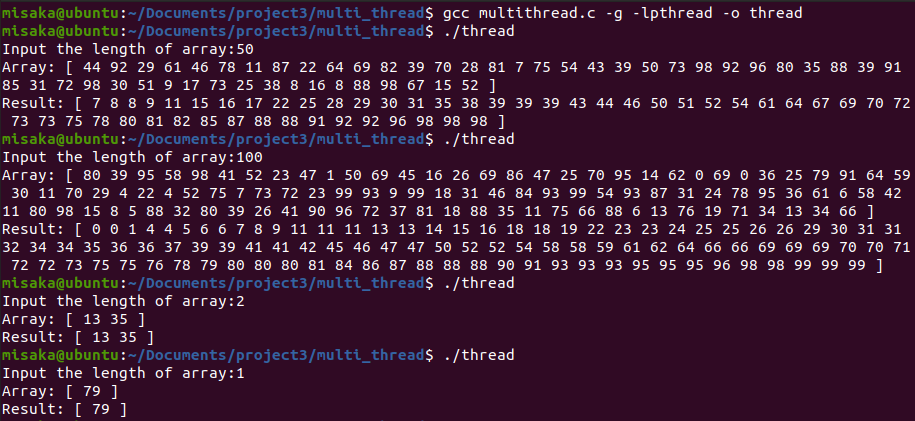
\includegraphics[width=400pt]{thread.png}
    \caption{Multithreaded Sorting}
    \label{3}
\end{figure}


\section{Fork-Join Sorting Application}

Implement the preceding project (Multithreaded Sorting Application) using
Java’s fork-join parallelism API. This project will be developed in two different versions. Each version will implement a different divide-and-conquer sorting algorithm:
\begin{itemize}
    \item QuickSort
    \item MergeSort
\end{itemize}

The Quicksort implementation will use the Quicksort algorithm for dividing
the list of elements to be sorted into a left half and a right half based on the position of the pivot value. The Mergesort algorithm will divide the list into two evenly sized halves. For both the Quicksort and Mergesort algorithms,
when the list to be sorted falls within some threshold value (for example, the
list is size 100 or fewer), directly apply a simple algorithm such as the Selection or Insertion sort. Most data structures texts describe these two well-known, divide-and-conquer sorting algorithms.  The source code download for this text includes Java code that provides the foundations for beginning this project.

\textbf{Design}: My design for this task is shown as follows:

\begin{itemize}
    \item \texttt{RecursiveAction} is extended to implement the sorting process
    \item In the \texttt{compute()} function, the concrete sorting algorithm is implemented and called recursively.
    \item If the length of array is less than \textbf{THRESHOLD}, the bubble sort is used to sort the array.
\end{itemize}

\subsection{QuickSort}

The code for Fork-Join QuickSort is shown as follows.
\begin{lstlisting}[language = java]
import java.util.concurrent.*;
import java.util.Scanner;

public class QuickSort extends RecursiveAction {
    private static final long serialVersionUID = 1L;
    static final int THRESHOLD = 10;
    private int start, end;
    private Integer[] array;

    public QuickSort(int start, int end, Integer[] array) {
        this.start = start;
        this.end = end;
        this.array = array;
    }

    protected void compute() {
        if (end - start < THRESHOLD) {
            for (int i = start; i < end; i++) {
                for (int j = i; j <= end; j++) {
                    if (array[i].compareTo(array[j]) > 0) {
                        Integer t = array[i];
                        array[i] = array[j];
                        array[j] = t;
                    }
                }
            }
        } else { // divide into sub-sort
            int mid = start + (end - start) / 2;
            Integer comp = array[start];
            int l, h;
            l = start;
            h = end;

            while (l < h) {
                while (l < h && array[h].compareTo(comp) >= 0) h--;
                if (l < h) array[l++] = array[h];
				while (l < h && array[l].compareTo(comp) <= 0) l++;
				if (l < h) array[h--] = array[l];
            }
            array[l] = comp;
            
            QuickSort taskl = new QuickSort(start, l - 1, array);
            QuickSort taskr = new QuickSort(l + 1, end, array);

            taskl.fork();
            taskr.fork();

            taskl.join();
            taskr.join();
        }
    }
    
    public static void main(String[] args) {
        ForkJoinPool pool = new ForkJoinPool();
        int n;

        Scanner input = new Scanner(System.in);
        System.out.print("Input the length of array:");
        n = input.nextInt();
        input.close();

        Integer[] array = new Integer [n];
        java.util.Random rand = new java.util.Random();

        System.out.print("Array: [ ");
        for (int i = 0; i < n; ++ i) {
            array[i] = rand.nextInt(1000);
            System.out.print(array[i] + " ");
        }
		System.out.println("]");	
        
        QuickSort task = new QuickSort(0, n - 1, array);
        pool.invoke(task);

        System.out.print("Result: [ ");
        for (int i = 0; i < n; ++ i) {
            System.out.print(array[i] + " ");
        }
		System.out.println("]");	
    }
}
\end{lstlisting}

The program can be compiled and executed with the following commands.

\begin{lstlisting}
javac QuickSort.java
java QuickSort
\end{lstlisting}


The result is shown as follows. The randomized array is sorted correctly by this program.
\begin{figure}[H]
    \centering
    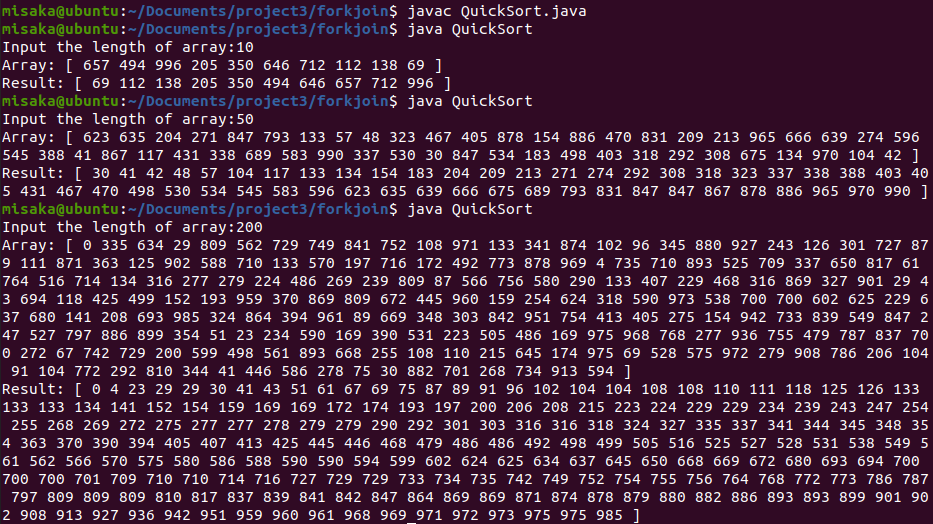
\includegraphics[width=400pt]{quick.png}
    \caption{Fork-Join QuickSort}
    \label{3}
\end{figure}

\subsection{MergeSort}

The code for Fork-Join QuickSort is shown as follows.
\begin{lstlisting}[language = java]
import java.util.concurrent.*;
import java.util.Scanner;

public class MergeSort extends RecursiveAction {
    private static final long serialVersionUID = 1L;
    static final int THRESHOLD = 10;
    private int start, end;
    private Integer[] array;

    public MergeSort(int start, int end, Integer[] array) {
        this.start = start;
        this.end = end;
        this.array = array;
    }

    protected void compute() {
        if (end - start < THRESHOLD) {
            for (int i = start; i < end; i++) {
                for (int j = i; j <= end; j++) {
                    if (array[i].compareTo(array[j]) > 0) {
                        Integer t = array[i];
                        array[i] = array[j];
                        array[j] = t;
                    }
                }
            }
        } else { // divide into sub-merge
            int mid = start + (end - start) / 2;
            
            MergeSort taskl = new MergeSort(start, mid, array);
            MergeSort taskr = new MergeSort(mid + 1, end, array);

            taskl.fork();
            taskr.fork();

            taskl.join();
            taskr.join();

            Integer[] result = new Integer [end - start + 1];
            
            int loc1, loc2, i; // merge taskl and taskr
            loc1 = start;
            loc2 = mid + 1;
            i = 0;
            
            while (i < end - start + 1) {
                int flag = 1; // select which sub-array
                if (loc1 > mid) flag = 1;
                else if (loc2 > end) flag = 0; 
                else if (loc1 <= mid && (array[loc1] < array[loc2])) flag = 0;
                if (flag == 0) {
                    result[i++] = array[loc1++];
                } else {
                    result[i++] = array[loc2++];
                }
            }
            
            for (int j = 0; j < end - start + 1; j++) { // merge array from result
                array[start + j] = result[j];
            }
        }
    }
    
    public static void main(String[] args) {
        ForkJoinPool pool = new ForkJoinPool();
        int n;

        Scanner input = new Scanner(System.in);
        System.out.print("Input the length of array:");
        n = input.nextInt();
        input.close();

        Integer[] array = new Integer [n];
        java.util.Random rand = new java.util.Random();

        System.out.print("Array: [ ");
        for (int i = 0; i < n; ++ i) {
            array[i] = rand.nextInt(1000);
            System.out.print(array[i] + " ");
        }
		System.out.println("]");	
        
        MergeSort task = new MergeSort(0, n - 1, array);
        pool.invoke(task);

        System.out.print("Result: [ ");
        for (int i = 0; i < n; ++ i) {
            System.out.print(array[i] + " ");
        }
		System.out.println("]");	
    }
}
\end{lstlisting}



The program can be compiled and executed with the following commands.

\begin{lstlisting}
javac MergeSort.java
java MergeSort
\end{lstlisting}


The result is shown as follows. The randomized array is sorted correctly by this program.
\begin{figure}[H]
    \centering
    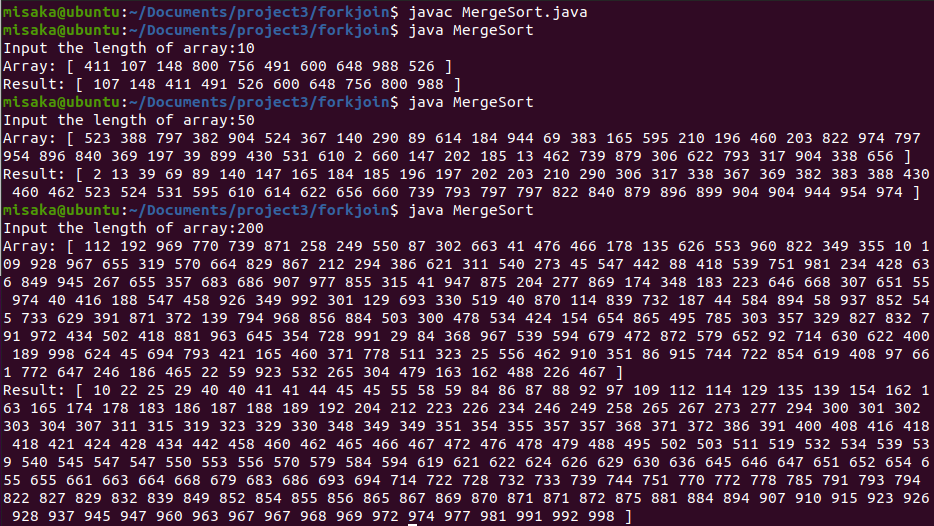
\includegraphics[width=400pt]{merge.png}
    \caption{Fork-Join MergeSort}
    \label{3}
\end{figure}
\end{document}